\documentclass[border=4pt]{standalone}
\usepackage{tikz}
\usetikzlibrary{arrows.meta}
\usepackage{eurosym}
\definecolor{citehl}{RGB}{255,224,102}
\definecolor{riskc}{HTML}{7C3AED}
\definecolor{effectc}{HTML}{0F766E}
\definecolor{posc}{HTML}{C2410C}
\definecolor{negc}{HTML}{1D4ED8}
\begin{document}
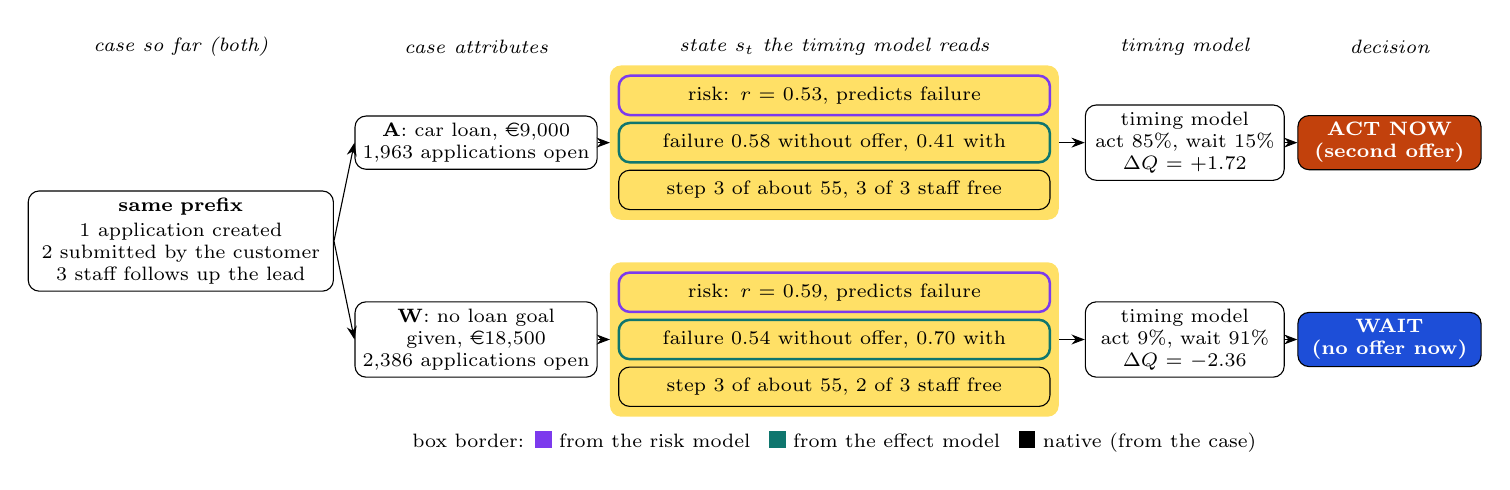
\begin{tikzpicture}[
  every node/.style={align=center, font=\scriptsize},
  box/.style={draw, rounded corners, inner sep=2.5pt, minimum height=0.5cm},
  >=Stealth
]
% el estado s_t de cada carril, resaltado como en fig1_retime.tex
\fill[citehl, rounded corners] (5.55,0.27) rectangle (11.25,2.23);
\fill[citehl, rounded corners] (5.55,-2.23) rectangle (11.25,-0.27);
\node[font=\scriptsize\itshape] at (8.4,2.4699999999999998) {state $s_t$ the timing model reads};
\node[box, text width=3.7cm] (prefix) at (0.1,0) {\textbf{same prefix}\\[1pt]1\ application created\\2\ submitted by the customer\\3\ staff follows up the lead};

% --- caso A: Application_381087716 ---
\node[box, text width=2.9cm] (attrA) at (3.85,1.25) {\textbf{A}: car loan, \euro{}9,000\\1,963 applications open};
\node[box, draw=riskc, line width=0.9pt, text width=5.3cm] (riskA) at (8.4,1.85) {risk: $r$ = 0.53, predicts failure};
\node[box, draw=effectc, line width=0.9pt, text width=5.3cm] (effA) at (8.4,1.25) {failure 0.58 without offer, 0.41 with};
\node[box, text width=5.3cm] (natA) at (8.4,0.65) {step 3 of about 55, 3 of 3 staff free};
\node[box, text width=2.35cm] (timA) at (12.85,1.25) {timing model\\act 85\%, wait 15\%\\$\Delta Q$ = +1.72};
\node[box, fill=posc, text=white, font=\scriptsize\bfseries, text width=2.15cm] (decA) at (15.45,1.25) {ACT NOW\\(second offer)};
\draw[->] (prefix.east) -- (attrA.west);
\draw[->] (attrA.east) -- (5.55,1.25);
\draw[->] (11.25,1.25) -- (timA.west);
\draw[->] (timA.east) -- (decA.west);


% --- caso W: Application_519115732 ---
\node[box, text width=2.9cm] (attrW) at (3.85,-1.25) {\textbf{W}: no loan goal given, \euro{}18,500\\2,386 applications open};
\node[box, draw=riskc, line width=0.9pt, text width=5.3cm] (riskW) at (8.4,-0.65) {risk: $r$ = 0.59, predicts failure};
\node[box, draw=effectc, line width=0.9pt, text width=5.3cm] (effW) at (8.4,-1.25) {failure 0.54 without offer, 0.70 with};
\node[box, text width=5.3cm] (natW) at (8.4,-1.85) {step 3 of about 55, 2 of 3 staff free};
\node[box, text width=2.35cm] (timW) at (12.85,-1.25) {timing model\\act 9\%, wait 91\%\\$\Delta Q$ = $-$2.36};
\node[box, fill=negc, text=white, font=\scriptsize\bfseries, text width=2.15cm] (decW) at (15.45,-1.25) {WAIT\\(no offer now)};
\draw[->] (prefix.east) -- (attrW.west);
\draw[->] (attrW.east) -- (5.55,-1.25);
\draw[->] (11.25,-1.25) -- (timW.west);
\draw[->] (timW.east) -- (decW.west);

% cabeceras
\node[font=\scriptsize\itshape] at (0.1,2.4699999999999998) {case so far (both)};
\node[font=\scriptsize\itshape] at (3.85,2.4699999999999998) {case attributes};
\node[font=\scriptsize\itshape] at (12.85,2.4699999999999998) {timing model};
\node[font=\scriptsize\itshape] at (15.45,2.4699999999999998) {decision};
% leyenda de niveles
\node[font=\scriptsize] at (8.4,-2.55) {box border:\enspace
  \textcolor{riskc}{\rule{6pt}{6pt}} from the risk model \enspace
  \textcolor{effectc}{\rule{6pt}{6pt}} from the effect model \enspace
  \rule{6pt}{6pt} native (from the case)};
\end{tikzpicture}
\end{document}
